%!TEX root = ../thesis.tex

\section{背景}
近年, ROS(Robot Operating System)をベースとした自律移動ロボットのナビゲーション技術が, 警備ロボットや案内ロボットなど, 様々な分野で活用されつつある. 
ただし, ナビゲーションにおいては, ROS Navigation stack\cite{navstack}のパラメータ, オドメトリ調整のパラメータ, 地図生成のパラメータなど, 複数のパラメータを
適切に調整しなければ自律移動を行うことができない. 

また, 現状ではこれらのパラメータ調整に関する明確な指針は十分に示されていない. 
特に, インターネット上で公開されている情報の多くは屋内環境を対象したものであり, 
センサ誤差や環境変動が大きく調整が困難な屋外環境に関連する情報は少ないという課題がある. 
そのため, 屋外環境にも対応したナビゲーションにおけるパラメータ調整手順の明確化が求められる. 
\newpage
\section{関連研究}
ROSのナビゲーションのパラメータ調整について解説されている関連研究として, Kaiyu Zheng\cite{zheng2017rosnavigation}によるROS Navigation Tuning Guideが挙げられる. 
このガイドは, ROS Navigation stackの性能を最大化するためのパラメータ調整プロセスを解説するものであり, AMCLやMove Baseなど, ナビゲーションにおける主要な項目を網羅している. 

しかし, \figref{Fig:laser-related parameters}, \figref{Fig:odometry and particle filter parameters}のように具体的なパラメータ値が提示され, それらが望ましい設定値であると示している. 
そのため, 自己位置推定のずれや経路計画の失敗など, 特定の環境や問題に直面した際に, どのパラメータをどのように調整すべきかという手順までは明確に示されていない. 
読み手はパラメータに関数する知見は得られるものの, 全体としてナビゲーションシステムを最適化していく具体的な調整フローを導き出すのは難しいという課題がある. 
\begin{figure}[hbtp]
  \centering
 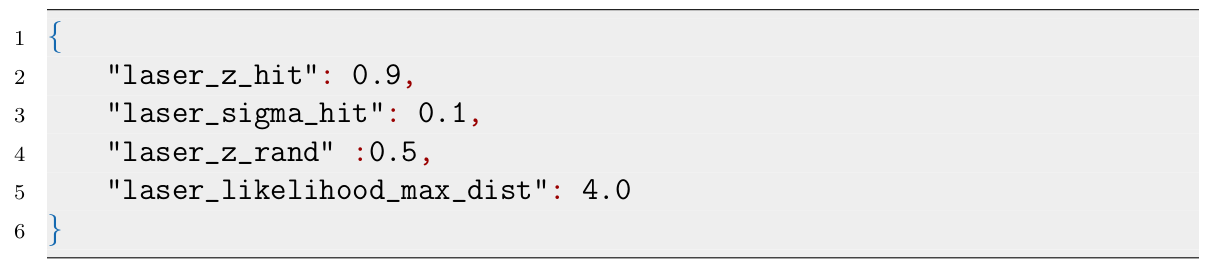
\includegraphics[keepaspectratio, scale=0.3]
      {images/senkou_1.png}
 \caption{laser-related parameters}
 \label{Fig:laser-related parameters}
\end{figure}

\begin{figure}[hbtp]
  \centering
 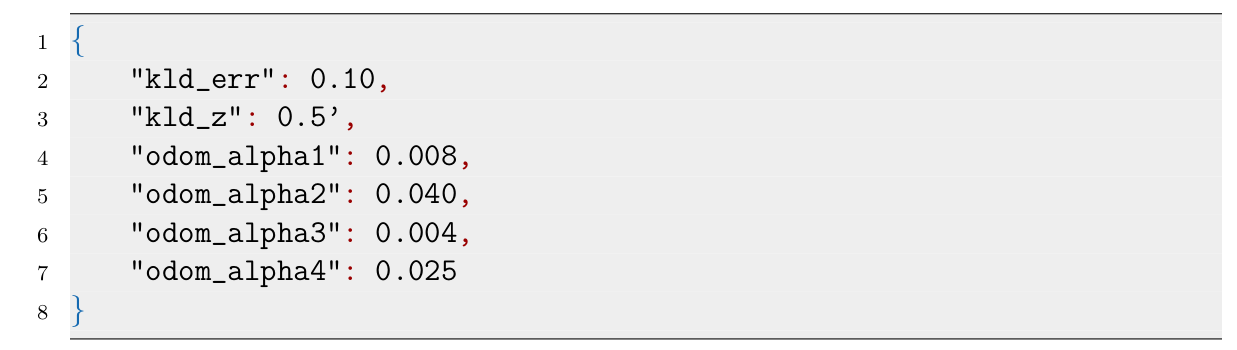
\includegraphics[keepaspectratio, scale=0.3]
      {images/senkou_2.png}
 \caption{odometry and particle filter parameters}
 \label{Fig:odometry and particle filter parameters}
\end{figure}
%\subsubsection{etc...}
\newpage
\section{目的}
本論文では, ロボットにおけるナビゲーションの調整手順を体系化し, 調整方法の一例を示すことを目的とする. 

\section{論文の構成}
本論文では以下のように構成される. 

2章で本研究で使用される要素技術について述べる. 

3章では本研究で作成したドキュメントについて述べる. 

4章では津田沼チャレンジによる実験でドキュメントの有効性を検証する. 

5章ではつくばチャレンジによる実験でドキュメントの有効性を検証する. 

6章では本論文について結論を述べる. 

\newpage
